%!TEX program = xelatex
\documentclass[11pt]{article}

\usepackage[dvipsnames]{xcolor} % needed to declare before tikz
\usepackage{amsmath,  latexsym, amssymb, url, amssymb, pgfplots, amsthm, mathtools, setspace, commath, tikz, verbatim, array, enumitem, bbding, bigints, fontspec, xunicode, xltxtra, geometry, algorithm, algpseudocode, graphicx,listings,lipsum,tabto,tcolorbox,sectsty,booktabs,siunitx,caption}
\usepackage[version=4]{mhchem}
\usepackage[utf8]{inputenc}


\NumTabs{6}

\defaultfontfeatures{Mapping=tex-text} 

\setmainfont{Charter} 

\newfontfamily\Codefont{Courier}  %{GillSans} %{AmericanTypewriter}

\definecolor{gry}{rgb}{.95,.95,.95}

\lstset{language=C++,
                moredelim=[is][\color{Green}\Codefont]{<}{>},
                basicstyle=\small\Codefont,
                identifierstyle=\Codefont,
                directivestyle=\color{BurntOrange}\Codefont,
                keywordstyle=\color{RubineRed}\Codefont,
                stringstyle=\color{Green}\Codefont,
                commentstyle=\color{gray}\Codefont,
                emphstyle=\color{Violet}\Codefont,
                emph={1,2,3,4,5,6,7,8,9,0},
                showspaces=false,
                %keywordstyle=[2]\color{Violet},
                keywords=[2]{*,1,2,3,4,5,6,7,8,9,0},
                keywordstyle=[2]\color{blue},
                showstringspaces=false,
                morecomment=[l][\color{orange}]{\#}}
\lstset{literate=%
    *{0}{{{\color{NavyBlue}0}}}1
    {1}{{{\color{NavyBlue}1}}}1
    {2}{{{\color{NavyBlue}2}}}1
    {3}{{{\color{NavyBlue}3}}}1
    {4}{{{\color{NavyBlue}4}}}1
    {5}{{{\color{NavyBlue}5}}}1
    {6}{{{\color{NavyBlue}6}}}1
    {7}{{{\color{NavyBlue}7}}}1
    {8}{{{\color{NavyBlue}8}}}1
    {9}{{{\color{NavyBlue}9}}}1
    {.0}{{{\color{NavyBlue}.0}}}2
    {.1}{{{\color{NavyBlue}.1}}}2
    {.2}{{{\color{NavyBlue}.2}}}2
    {.3}{{{\color{NavyBlue}.3}}}2
    {.4}{{{\color{NavyBlue}.4}}}2
    {.5}{{{\color{NavyBlue}.5}}}2
    {.6}{{{\color{NavyBlue}.6}}}2
    {.7}{{{\color{NavyBlue}.7}}}2
    {.8}{{{\color{NavyBlue}.8}}}2
    {.9}{{{\color{NavyBlue}.9}}}2
}
\lstset{alsolanguage=[90]Fortran}
\lstset{alsolanguage=python}
\lstset{backgroundcolor=\color{gry}}
\lstset{frame=single}
\lstset{
    numbers=left,
    numberstyle=\Codefont,
    title=\lstname,
    tabsize=4,
}
\geometry{margin=1in}
\geometry{letterpaper} % or letterpaper (US) or a5paper or....
\usepackage[parfill]{parskip} % Activated to begin paragraphs with an empty line rather than an indent

\title{PHY 480 - Computational Physics \\ Project 1: Linear Algebra Methods}
\author{Thomas Bolden}
\date{February 12, 2016}

\usepackage{hyperref}
\hypersetup{
    colorlinks=true,
    linkcolor=darkgray,
    filecolor=magenta,      
    urlcolor=Emerald,
}

\setcounter{secnumdepth}{0} % deactivate for section numbers
%\sectionfont{\fontsize{12}{15}\selectfont} % Activate for same font size sections
\subsectionfont{\fontsize{15}{15}\selectfont}
\newenvironment{amatrix}[1]{%
  \left[\begin{array}{@{}*{#1}{c}|c@{}}
}{%
  \end{array}\right]
}

\setmainfont{Charter}

\begin{document}

%\tableofcontents
\maketitle

\thispagestyle{empty}

\centerline{Github Repository at \href{https://github.com/ThomasBolden/PHY-480-Spring-2016}{https://github.com/ThomasBolden/PHY-480-Spring-2016}}

\begin{abstract}

    In this project, a solution was found to the one-dimensional Poissson equation with Dirichlet boundary conditions. This was done by rewriting the Poisson equation as a set of linear equations and implimenting a tridiagonal matrix solver. It was confirmed that the tridiagonal solver approximation became more accurate as the step size decreased. Then, two other methods (Gaussian elimination, and LU decomposition) were implemented and compared. The error in the results of the LU defactorization method were found to be smaller than the error in the Gaussian elimination method.However, the calculation time became impractical after $n=$ steps.

\end{abstract}

\vspace{\fill}
\tableofcontents

 \vspace{2cm}

\pagebreak

\setcounter{page}{1}

\subsection{Introduction}

    An important skill in physics is being able to efficiently solve differential equations. There are many situations in which differential equations can be solved as a system of linear equations. Such equations are called linear second-order differential equations, of the form
    \begin{equation} \dfrac{\dif\,^2 y}{\dif x^2} + k^2(x) y = f(x) \; , \end{equation}
    where $f(x)$ is the inhomogenous term, and $k^2$ is a real function. \\

    An example of this being useful is in electromagnetism. Poisson's equation describes the electrostatic potential energy field $\Phi$ caused by a given charge density distribution $\rho$. The equation in three dimensions is
    \begin{equation} \nabla^2 \Phi = - 4 \pi \rho(\mathbf{r}) \end{equation}
    where the electrostatic potential and charge density are spherically symmetric. This allows one to simplify the equation to one dimension 
    \begin{equation} \dfrac{1}{r^2} \dfrac{\dif}{\dif r} \left( r^2 \dfrac{\dif \Phi}{\dif r} \right) = -4\pi \rho(r) \end{equation}
    which can be rewritten using the substitution $\Phi (r) = \phi (r) /r$
    \begin{equation} \dfrac{\dif\,^2 \phi}{\dif{r^2}} = -4\pi r \rho(r). \end{equation}
    Now, like equation (1), this is linear second order in $r$. This becomes clear when we let $k^2(r)=0$ , $f(r)=-4\pi r \rho(r)$. If we let $\phi \to u$ and $r \to x$, we get the general Poisson equation
    \begin{equation} -u'' = f(x). \end{equation}
    If we apply certain boundary conditions, we can rewritten as a set of linear equations. In this project, I explored several methods of solving systems of linear equations, including Gaussian elimination, LU decomposition, and analytically. In the section that follows, I outline the methods and algorithms used to write the C++ code, along with some examples of the output one should expect when running the code themself. The next section contains the useful results. In it, I compare the run times and efficiency of each method used, along with the magnitude of the associated error. Finally, the source code is presented for reference.

\subsection{Methods}

    Given a differential equation of the form 
    \begin{equation} - \dfrac{\dif\,^2}{\dif x^2} u(x) = f(x) \end{equation}
    where $f(x)$ is continuous on the domain $x \in (0,1)$. We also assume the Dirichlet boundary conditions $u(0)=u(1)=0$. We can define a discretized approximation second derivative of $u$ as $v_i$ with grid points $x_i=ih$ in the interval $x_0=0$ to $x_{n+1}=1$, and with step lengths $h=1/(n+1)$. The boundary conditions become $v_0 = 0 = v_{n+1}$. If the source term is $f(x) = 100e^{-10x}$ , the exact closed-form solution is $u(x) = 1−(1−e^{−10})x−e^{−10x}$. The second derivative of $u$ can be approximated as 
    \begin{equation} -u'' = -\dfrac{v_{i+1}+v_{i-1}-2v_i}{h^2} = f_i \;\;\;\; \text{for}\;\; i = 1,\dots,n \end{equation}
    This equation can be written as a set of linear equations of the form
    \begin{equation} \mathbf{Av} = \tilde{\mathbf{b}}  \end{equation}
    

    \[ \arraycolsep 1.0ex \mathbf{A} = \left[ \begin{array}{c c c c c c c} 
    \vspace{.1cm} 2 & \llap{-}1 & 0 & \cdots & \cdots & \cdots & 0 \\
    \llap{-}1 & 2 & \llap{-}1 & 0 & \cdots & \cdots & 0 \\
    0 & \llap{-}1 & 2 & \llap{-}1 & \ddots &  & \vdots \\
    \vdots & 0 & \llap{-}1 & 2 & \ddots & \ddots & \vdots \\
    \vdots & \vdots & \ddots &\ddots&\ddots&\ddots&0 \\
    \vdots &\vdots&&\ddots&\ddots&\ddots& \llap{-}1 \vspace{.1cm} \\ 
    0 &0&\cdots&\cdots&0&\llap{-}1& 2 
    \end{array} \right] \;\; , \;\; \bold{v} = \left[ \begin{array}{c} v_0 \\ v_1 \\ \vdots \\ \vdots \\ v_{n-1} \\ v_n \end{array} \right] \;\; , \;\; \tilde{b}_i = h^2 f_i \]

    One way to solve tridiagonal matrices (like the one above) is Gaussian elimination. Basically, Gaussian elimination uses the first equation to eliminate the first unknown $x_1$ from the remaining equations, and continues this trend for the remaining equations until an upper triangular matrix is formed. An upper triangular matrix can be easily solved using back substitution. This process requires a total of $\mathcal{O}(8n)$ floating point operations. The general algorithm is below.
    
    \begin{algorithm}
    \caption{Gaussian Elimination}
    \label{Gaussian Elimination}
    \begin{algorithmic}[1]
    \Function{GaussElim}{A}
    \For{$k=1$ to  $n-1$}
    \For{$i=k+1$ to $n$}
    \State $a_{ik} = \frac{a_{ik}}{a_{kk}}$
    \For{$j=k+1$ to $n+1$}
    \State $a_{ij}=a_{ij}-a_{ik}\times a_{kj}$
    \EndFor
    \EndFor
    \EndFor
    \EndFunction
    \end{algorithmic}
    \end{algorithm}

    We can compare this algorithm to the standard lower-upper (LU) decomposition. Equation (8) can also be written as $\mathbf{A}=LU$, assumin $\mathbf{A}$ is invertible. 
    \begin{equation}
    \mathbf{A} = \left[ \begin{array}{ccccc} 1&0&\cdots &\cdots &0\\ l_{21} & 1 & 0 & \cdots & 0 \\ l_{31} & l_{32} & \ddots & \ddots & \vdots \\ \vdots &\vdots &\ddots & \ddots &0 \\ l_{n1} &l_{n2} &\cdots & l_{n,n-1}& 1 \end{array} \right] \left[ \begin{array}{ccccc} u_{11} & u_{12} &\cdots &\cdots &u_{1n} \\ 0&u_{22}&\ddots&&\vdots \\ \vdots&0&\ddots&\ddots&\vdots \\ \vdots&\vdots&\ddots&\ddots&u_{n-1,n} \\ 0&0&\cdots&0&u_{nn} \end{array} \right]
    \end{equation}

    \begin{algorithm}
    \caption{LU Decomposition}
    \label{LU Decomp}
    \begin{algorithmic}[1]
    \Function{LUdecomp}{A}
    \For{$i=1$ to  $n$}
    \For{$j=i$ to $n$}
    \State $L_{ik}U{kj}=a_{ij}$
    \EndFor
    \For{$j=i+1$ to $n$}
    \State $L_{jk}U_{ki}=a_{ji}$
    \EndFor
    \EndFor
    \EndFunction
    \end{algorithmic}
    \end{algorithm}

    This requires approximately $\frac{2}{3}n^3$ floating point operations on an $n$ by $n$ matrix. \pagebreak

    The final task is to time each of the algorithms above. This is done most easily using the ``time.h'' header in C++.

    

\subsection{Results}

    The graph below shows how the accuracy of the traditional tridiagonal matrix solver increases as the step length increases.

    \begin{figure}[h!] \begin{center}
    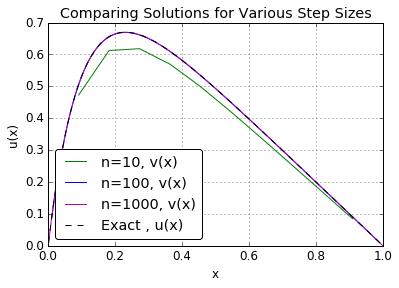
\includegraphics{setpsizechange.png}
    \end{center}  \end{figure}

\pagebreak
\subsection{Conclusions}

    I have show how the accuracy of the solution to a linear system depends on the size of the system. For smaller systems, the number of floating point operations did not impede the ability of the user to impliment more accurate methods.

\subsection{Code}

    \lstinputlisting[language=C++]{../Code/Project1.cpp}

    \lstinputlisting[language=python]{../Code/plots.py}

\begin{thebibliography}{1}

    \bibitem{morten} M. Hjorth-Jensen, {\em Computational Physics}, University of Oslo (2013).

    \bibitem{mclean} W. McLean, {\em Poisson Solvers}, Northwestern University (2004).

\end{thebibliography}














\end{document}